\chapter{转发引擎}\label{forward}

\section{简介}
转发引擎主要负责以下5种工作:
\vspace{-8pt}
\begin{enumerate}
	\item 向下一跳传递包,在需要时重传,同时根据是否收到ACK向链路估计器传递相应信息。
	\item 决定何时向下一跳传递包
	\item 检测路由中的不一致性,并通知路由引擎
	\item 维护需要传输的包队列,它混杂了本地产生的包和需要转发的包。
	\item 检测由于丢失ACK引起的单跳重复传输
\end{enumerate}

\section{基本概念}
\subsection{路由循环}
路由循环是指某个节点将数据包转发给下一跳,而下一跳节点是它的子孙节点或者它本身,从而造成了数据包
在该环路中不断循环传递,如图\ref{route-loop}所示,由于节点E在某个时刻错误地选择了H节点作为父节点,从而造成了路由循环。

\begin{figure}[ht]
\centering
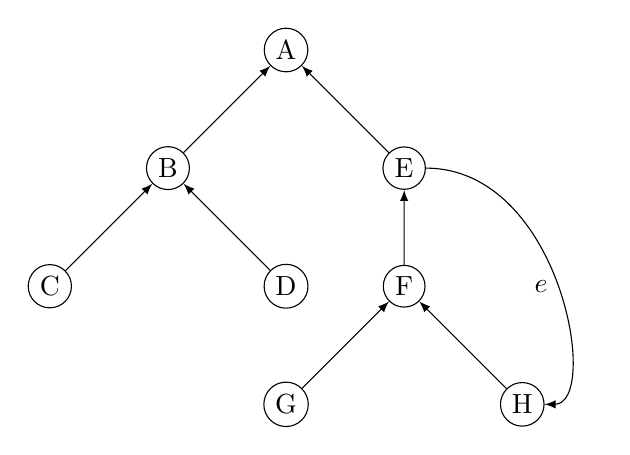
\begin{tikzpicture}[>=latex,level/.style={sibling distance=3cm}]
	\node[circle,draw,inner sep=2] {A}
		child[<-] {node[circle,draw,inner sep=2] {B}
			child {node[circle,draw,inner sep=2] {C}}
			child {node[circle,draw,inner sep=2] {D}}
		}
		child[<-] {node[circle,draw,inner sep=2] (E) {E}
			child {node[circle,draw,inner sep=2] {F}
				child {node[circle,draw,inner sep=2] {G}}
				child {node[circle,draw,inner sep=2] (H) {H}}
			}
		};
	\draw[->] (E) .. controls +(right:2) and +(right:1) .. node[left] {$e$}(H);
\end{tikzpicture}


\caption{路由循环}\label{route-loop}
\end{figure}

\subsection{包重复}
包重复是指节点多次收到具有相同内容的包。这主要是由于包重传引起的。比如发送者发送了一个数据包,
接收者成功地收到了该数据包并回复ACK,但ACK在中途丢失,因此发送者会将该包再一次发送,从而在
接收者处造成了包重复现象。

\subsection{CTP数据帧}
CTP数据帧是转发引擎在发送本地数据包时所使用的格式。它在数据包头增加一些字段用于抑制包重复和路由循环。

CTP数据帧格式如图\ref{ctp-data-frame}所示:
\begin{figure}[ht]
\centering
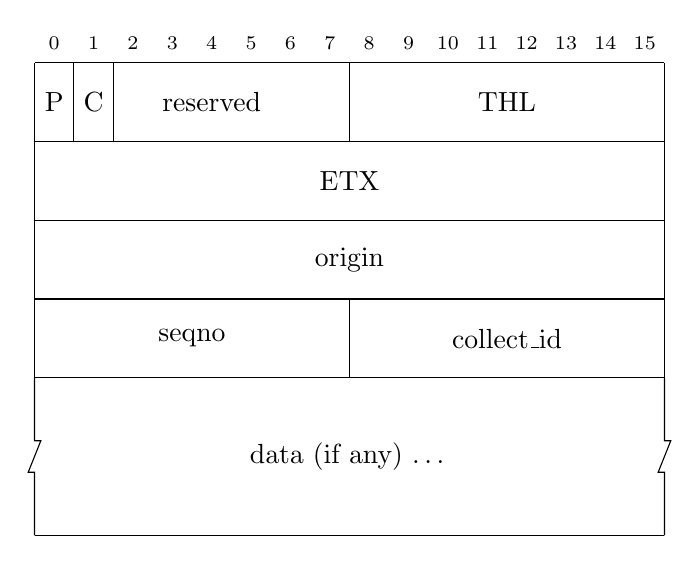
\begin{tikzpicture}
\pagella
	\draw (0,-1) -- (8,-1);
	\draw (0,1) -- (8,1);
	\draw (0,2) -- (8,2);
	\draw (0,3) -- (8,3);
	\draw (0,4) -- (8,4);
	\draw (0,5) -- (8,5);

	\draw (0,1) -- (0,5);
	\draw (8,1) -- (8,5);

	%\draw (0,0) -- (0,0.4) -- (-0.08,0.4) -- (0.08,0.6) -- (0,0.6) -- (0,1);
	\draw (0,-1) -- (0,-0.2) -- (-0.08,-0.2) -- (0.08,0.2) -- (0,0.2) -- (0,1);
	%\draw (8,0) -- (8,0.4) -- (8-0.08,0.4) -- (8+0.08,0.6) -- (8,0.6) -- (8,1);
	\draw (8,-1) -- (8,-0.2) -- (8-0.08,-0.2) -- (8+0.08,0.2) -- (8,0.2) -- (8,1);

	\draw (0.5,4) -- (0.5,5);
	\draw (1,4) -- (1,5);
	\draw (4,4) -- (4,5);
	\draw (4,1) -- (4,2);

	\foreach \x in {0,...,15}
	{
	  \draw (\x*0.5+0.25,5.25) node {\scriptsize \x};
	}
	\draw (0.25,4.5) node {P};
	\draw (0.75,4.5) node {C};
	\draw (2.25,4.5) node {reserved};
	\draw (6,4.5) node {THL};
	\draw (4,3.5) node {ETX};
	\draw (4,2.5) node {origin};
	\draw (2,1.5) node {seqno};
	\draw (6,1.5) node {collect\_id};
	\draw (4,0) node {data (if any) \ldots};
\end{tikzpicture}
\caption{CTP数据帧格式}\label{ctp-data-frame}
\end{figure}

各字段定义如下:
\vspace{-10pt}
\begin{itemize}
	\item P:取路由位。P位允许节点从其它节点请求路由信息。
		如果节点收到一个P位置位的包,它应当传输一个路由帧。
	\item C:拥塞标志位。如果节点丢弃了一个CTP数据帧,
		它必须在下一个传输的数据帧中置C位。
	\item THL:已存活时间(Time Have Lived),它主要用于解决路由循环问题。
		当节点产生一个CTP数据帧时,
		它必须设THL为0。当节点接收到一个CTP数据帧时,
		它必须增加THL值。如果节点接收到的数据包THL为255,则将它回绕为0。
		该字段主要用于解决数据包在环路中停留太久的问题,
		但在当前版本的CTP协议中暂时还没有实现这一功能。
	\item ETX:单跳发送者的ETX值。当节点发送一个CTP数据帧时,
		它必须将到单跳目的地的路由ETX值填入ETX字段。
		如果节点接收到的路由梯度比自己的小,则它必须准备发送一个路由帧。
	\item origin:包的源地址。转发的节点不可修改这个字段。
	\item seqno:源顺序号。源节点设置了这个字段,转发节点不可修改它。
	\item collect\_id:高层协议标识。源节点设置了这个字段,转发节点不可修改它。
	\item data:数据负载。0个或多个字节。转发节点不可修改这个字段。
\end{itemize}
\vspace{-10pt}

origin,~seqno,~collect\_id合起来标识了一个唯一个源数据包,
而origin,~seqno,~collect\_id,~THL合起来标识了网络中唯一一个数据包实例。
两者的区别在路由循环中的重复抑制是很重要的。如果节点抑制源数据包,
则它可能丢弃路由循环中的包;如果它抑制包实例,则它允许转发处于短暂
的路由循环中的包,除非THL凑巧回绕到与上次转发时相同的状况。

\subsection{队列项}
队列项(Queue Entry)中存放了对应消息的指针、对应的发送者和可重传次数。本地包与转发包的队列项分配方法有所不同:转发包的队列项是通过缓冲池分配的,而本地包的队列项是编译期间静态分配的。

\subsection{消息发送队列}
消息发送队列结构是转发引擎的核心结构。它存放了队列项的指针,
队头元素指向的队列项中的消息将被优先发送。

\subsection{缓冲池}
缓冲池是操作系统中用于统一管理缓冲区分配的一个设施\ucite{bach1986duo}。
应用程序可以使用缓冲池提供的接口方便地获取和释放缓冲区。
对于不能动态分配存储空间的TinyOS来说,这一点非常有价值,因为它可以重复
利用一段静态存储空间。

转发引擎中使用了两个缓冲池:队列项缓冲池(QEntryPool)和消息缓冲池
(MessagePool)。队列项缓冲池用于为队列项分配空间,如图\ref{qe-buffer-pool}所示,
当转发引擎收到一个需要转发的消息时,它会从队列项缓冲区中取出一个空闲的队列项,
作相应的初始之后把队列项的指针放入消息队列队尾。在成功地发送了一个
消息并收到ACK或消息重发次数过多被丢弃时,转发引擎会从队列项缓冲池中
释放这个消息对应的队列项,使它变为空闲,因此队列缓冲池就可以把这块
空间分配给后续的消息。

\begin{figure}[ht]
\centering
\begin{tikzpicture}[>=latex]
	\fill[gray!40] (2,4) rectangle (3,3.5);
	\fill[gray!40] (2,2.5) rectangle (3,2);
	\draw (2,4) rectangle (3,2);
	\draw (2,2.5)--(3,2.5);
	\draw (2,3)--(3,3);
	\draw (2,3.5)--(3,3.5);
	\node at (2.5,3.75) {0};
	\node at (2.5,3.25) {1};
	\node at (2.5,2.75) {2};
	\node at (2.5,2.25) {3};

	\fill[gray!40] (7,3.5) rectangle (8,3);
	\fill[gray!40] (7,2) rectangle (8,1.5);
	\fill[gray!20] (7,2.5) rectangle (8,2);
	\draw (7,3.5) rectangle (8,1.5);
	\draw (7,3)--(8,3);
	\draw (7,2.5)--(8,2.5);
	\draw (7,2)--(8,2);
	\node at (7.5,3.25) {0};
	\node at (7.5,2.75) {1};
	\node at (7.5,2.25) {2};
	\node at (7.5,1.75) {3};

	\fill[gray!40] (5,8) rectangle (6,7.5);
	\fill[gray!40] (5,6.5) rectangle (6,6);
	\fill[gray!40] (5,7) rectangle (6,6.5);
	\draw (5,8) rectangle (6,6);
	\draw (5,7.5)--(6,7.5);
	\draw (5,7)--(6,7);
	\draw (5,6.5)--(6,6.5);
	\node at (5.5,7.75) {0};
	\node at (5.5,7.25) {1};
	\node at (5.5,6.75) {2};
	\node at (5.5,6.25) {3};
	
	%\draw[rotate=-10] (2,3.4) ellipse (1.2 and 1.5);
	%\draw[rotate=-10] (7,3.7) ellipse (1.2 and 1.5);
	%\draw[rotate=-10] (4.2,7.8) ellipse (1.2 and 1.5);

	\node (AI) at (2,2.75) {};
	\node (AO) at (3,2.75) {};
	\node (BI) at (7,2.25) {};
	\node (BO) at (8,2.25) {};
	\node (CI) at (6,6.6) {};
	\node (CO) at (5,6.75) {};

	\draw[->] (AO) .. controls +(right:2) and +(left:1) .. node[below] {获取qe} (BI);
	\draw[->] (BO) .. controls +(right:2) and +(right:2) .. node[right] {使用qe} (CI);
	\draw[->] (CO) .. controls +(left:2) and +(left:2) .. node[left] {释放qe} (AI);

	\draw (7,7.3) -- node[above] {\footnotesize 将qe指针放入发送队列} (9,7.3);
	\draw (7,6.7) -- (9,6.7);
	\draw (7.5,7.3) -- (7.5,6.7);
	\draw (7.9,7.3) -- (7.9,6.7);
	\draw (8.3,7.3) -- (8.3,6.7);
	\draw (8.7,7.3) -- (8.7,6.7);
	\node at (7.7,7) {2};
	\node at (8.1,7) {0};
	\node at (8.5,7) {3};
	\draw[->] (6,6.8) .. controls +(right:0.8) and +(left:0.5).. (7.3,7);
\end{tikzpicture}

\caption{从缓冲池分配和释放队列项}\label{qe-buffer-pool}
\end{figure}

消息缓冲池的工作原理与队列项缓冲池类似,只不过它存的是消息结构。
消息缓冲池有一个缓冲区交换的行为,在“缓冲区交换”一节中详细论述。

在TinyOS 2.x中,消息缓冲池的初始大小设定为一个常数FORWARD\_COUNT(值为12)。
队列项缓冲池的初始大小为CLIENT\_COUNT + FORWARD\_COUNT,
其中CLIENT\_COUNT是CollectionSenderC使用者的个数,加上它是考虑到了本地
产生的包也会进入发送队列,而本地包的最大个数正是CollectionSenderC使用者
的个数,这样就保证了发送队列不会因为本地发送者太多而不断产生溢出。
如果不考虑这个因素,则在本地发送者很多的情况下节点可能产生拥塞的假象。

\subsection{缓冲区交换}\label{bufswap}
缓冲区交换是转发过程中一个比较微妙的环节。如图\ref{buffer-swap}所示,
从缓冲池中获得的消息结构并不是直接用于存储当前接收到的消息,而是用于
存储下一次收到的消息。由于当前接收到的消息必定已经有了它自己的存储空间,
因此只要让相应的队列项指向它就可以找到这个消息的实体。但是下一个接收到的消息就不应该
存储在这一块空间,而缓冲区交换正是用于为下一次收到的消息分配另外一块
空闲的存储空间。传统的做法通常是设置一个消息结构用于接收消息,
每当收到一个消息后将它整个复制到空闲存储空间中。相比之下,缓冲区交换
可以省去一次复制的开销。

\begin{figure}[ht]
\centering
\begin{tikzpicture}[>=latex]
	\usetikzlibrary{shapes}
	\node[ellipse,draw] (BP) at (4,1.5) {缓冲池};
	\node[ellipse,draw] (MP) at (8,3.5) {队列项};
	\node[rectangle,draw] (BF) at (4,5.5) {缓冲区};
	\node[rectangle,draw] (RC) at (4,7) {接收器};

	\draw[->] (BP) .. controls +(left:2)  and +(left:2) .. node[left] {获取msg} (BF);
	\draw[->] (BF) .. controls +(right:2) and +(up:1.5) .. node[above,rotate=-20] {使用msg} (MP);
	\draw[->] (MP) .. controls +(down:1) and +(right:2) .. node[below,rotate=30] {释放msg} (BP);
	\draw[->] (RC) -- node[right] {填充msg} (BF);
\end{tikzpicture}

\caption{缓冲区交换}\label{buffer-swap}
\end{figure}

\section{实现}
组件\texttt{tos/lib/net/ctp/CtpForwardingEngineP.nc}实现了转发引擎。

\subsection{使用的接口和提供的组件}
从下列源码中可以看到,CtpForwardingEngine使用了路由引擎提供的接口UnicastNameFreeRouting用于得到下一跳信息,使用了系统提供的Queue、Pool、SendCache接口分别实现消息发送队列、队列项缓冲池、消息缓冲池和发送消息缓存,同时也使用了LinkEstimator用于向链路估计器反馈数据包发送成功与否的信息。

%\begin{lstlisting}[captionpos=b,caption={\song CtpForwardingEngineP组件使用和提供的接口},label=ctp-forward-engine]
\begin{lstlisting}
generic module CtpForwardingEngineP() {
	provides {
		interface Init;
		interface StdControl;
		interface Send[uint8_t client];
		interface Receive[collection_id_t id];
		interface Receive as Snoop[collection_id_t id];
		interface Intercept[collection_id_t id];
		interface Packet;
		interface CollectionPacket;
		interface CtpPacket;
		interface CtpCongestion;
	}
	uses {
		interface AMSend as SubSend;
		interface Receive as SubReceive;
		interface Receive as SubSnoop;
		interface Packet as SubPacket;
		interface UnicastNameFreeRouting;
		interface SplitControl as RadioControl;
		interface Queue<fe_queue_entry_t*> as SendQueue;
		interface Pool<fe_queue_entry_t> as QEntryPool;
		interface Pool<message_t> as MessagePool;
		interface Timer<TMilli> as RetxmitTimer;
		interface LinkEstimator;
		interface Timer<TMilli> as CongestionTimer;
		interface Cache<message_t*> as SentCache;
		interface CtpInfo;
		interface PacketAcknowledgements;
		interface Random;
		interface RootControl;
		interface CollectionId[uint8_t client];
		interface AMPacket;
		interface CollectionDebug;
		interface Leds;
	}
}
\end{lstlisting}

CtpForwardingEngine提供的接口分别为网络中的四种扮演不同角色的节点服务。为发送者提供Send接口,为侦听者提供Snoop接口,为网络处理者提供Intercept接口,为接收者提供Receive接口。

\subsection{关键函数}
转发引擎的四个关键函数为包接收SubReceive.receive(),包转发forward(),
包传输SendTask()和包传完之后的善后工作SubSend.sendDone()。

\subsubsection{receive()函数}
receive()函数决定节点是否转发一个包。它有一个缓冲区缓存了最近收到的包,
通过检查这个缓冲区可以确定它是否是重复的。如果不是,则调用forward()函数
进行转发。

\subsubsection{forward()函数}
forward()函数格式化需要转发的包。它检查收到的包是否有路由循环,使用的方法是判断包头中的ETX值是否比本节点的路径ETX小。接着检查发送队列中是否有足够的空间,如果没有,则丢弃该包并置C位。如果传输队列为空,则投递SendTask任务准备发送。

\subsubsection{SendTask任务}
SendTask任务检查位于发送队列队头的包,请求路由引擎的路由信息,为到下一跳的传输作好准备,
并将消息提交到AM层。

\subsubsection{sendDone事件}
当发送结束时,sendDone事件处理程序会检查发送的结果。如果包被确认,则将包从传输队列中取出。
如果包是本地产生的,则将sendDone信号向上传。如果包是转发的,则将该消息结构释放到
消息缓冲池。如果队列中还有剩余的包(比如没有被确认的),它启动一个随机定时器
以重新投递这个任务。该定时器实质上用于限制CTP的传输速率,不让它尽快地发包,
这是为了防止在通路上自我冲突。

\subsection{工作流程分析}
当转发引擎收到一个转发包时,它会检查该数据包是否在缓存或发送队列中,
这主要是为了抑制包重复。如果不是重复包,则调用forward()进行转发。forward()函数为该消息
在消息池中分配队列项和消息结构,然后把队列项指针放入发送队列。如果此时投递
发送消息任务的定时器没有运行,则立即投递发送消息任务,
以选取发送队列队头的数据包进行发送。发送成功之后将触发sendDone
事件做一些善后工作,比如检查刚发送的包是否收到链路层ACK,
如果收到,则从队列中删除这个包的队列项,并释放相关资源。如果
没有收到ACK,则启动重传定时器,再一次投递发送消息任务进行重传。
若重传次数超过CLIENT\_COUNT次,则丢弃该包。

\subsection{本地数据包的发送}
转发引擎也负责本地数据包的发送。应用程序通过使用CollectionSenderC
组件发送本地包。nesC编译器会根据CollectionSenderC组件使用者的
个数为每个使用者静态地分配一个队列项,并用一个指针数组指向各自的队列项。
如果某个使用者需要发送数据包,则先检查它对应的指针是否为空。若为空,
则说明该使用者发送的前一个数据尚未处理完毕,返回发送失败;若不为空,
则说明它指向的队列项可用,用数据包的内容填充队列项并把它放入发送队列等待发送。
